\chapter{How to Write a Bestselling Novel}

This lecture begins in a room and then quickly refuses to let the room become the point. The den, the shelves, the secret door, even the aura of where ``the magic happens'' are all reduced to prelude. What matters is process: how drafts are arranged, how criticism is absorbed, why rewriting is treated as a full reconstruction rather than a cleanup pass, and how one continues through the moment when a book seems to collapse under its own length.

\section{The Room, and the Immediate Turn Away from It}

The interview opens with atmosphere. We are shown the den, the hidden door, and the spot where the books are made. But the lecturer immediately demystifies the setting: one can write in an airport lounge, on a plane, in a car. The room is good, perhaps the best place, but not the essential thing.

That opening matters because it prevents us from taking the wrong lesson. The lecture is not about sanctifying a writing chamber. It is about method. The room is merely the point of entry into a more serious question: what is the actual process by which a book gets written and rewritten?

\subsection{Question \& Answer}

\paragraph{Question.} Does a writer need the ideal room, or only a working process?

\paragraph{Answer.} The lecture's answer is clear. A good room helps, but it is not decisive. The real determinant is a repeatable method. The room is atmosphere; the process is structure.

\section{Three Screens and the Logic of Revision}

Once the room is set aside, the lecture becomes procedural. The interviewer asks about the three screens, and at once the work is laid out as a visible flow of information. One screen shows the first draft. Another shows comments from readers who have seen that draft. In the middle is the second draft in progress.

The arrangement can be compressed into the lecture's first central relation:
\begin{equation}
\text{first draft} \to \text{reader comments} \to \text{second draft}.
\end{equation}
This is not a mechanical sequence only; it is an epistemology of revision. The writer does not simply produce text and admire it. The draft is exposed to response, the response is interpreted, and the new draft is built under the pressure of that interpretation.

We can sharpen the same point in a second form:
\begin{equation}
\text{reader response} \to \text{diagnosis} \to \text{revision priority}.
\end{equation}
A comment does not matter merely because someone said it. It matters because it may reveal where the manuscript is not doing what it thinks it is doing.

\begin{figure}[h]
\centering
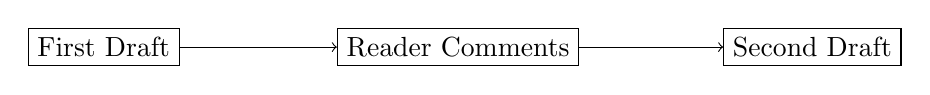
\begin{tikzpicture}
\node[draw, rectangle] (A) at (0,0) {First Draft};
\node[draw, rectangle] (B) at (4.5,0) {Reader Comments};
\node[draw, rectangle] (C) at (9,0) {Second Draft};
\draw[->] (A) -- (B);
\draw[->] (B) -- (C);
\end{tikzpicture}
\end{figure}

This schematic is deliberately plain. There is no validated frame of the monitor layout to preserve, so the figure is transcript-based rather than visually extracted. But it captures the lecture's central insight: revision is not a vague polishing mood, but an ordered flow from manuscript to response to reconstruction.

\subsection{Question \& Answer}

\paragraph{Question.} What information belongs in front of the writer while revising?

\paragraph{Answer.} The lecture answers by arrangement: the existing draft, the responses it has provoked, and the space where the next draft is being made. Revision works best when these are held in explicit relation to one another.

\section{Comments, Pace, and the Plot-Twist Heuristic}

The lecture then shows the method at work on a specific comment. One reader says that they were not drawn in as quickly and did not read as fast as with the previous books. Follett does not take this as an injury. He treats it as evidence. The inference is immediate:
\begin{equation}
\text{not drawn in quickly} \Rightarrow \text{opening chapter may be ponderous}.
\end{equation}
From there the diagnosis is generalized into a pacing rule:
\begin{equation}
\text{plot twist interval} \approx 3\text{--}4 \ \text{pages}.
\end{equation}
This is one of the lecture's clearest quantitative claims. It is not offered as universal law, but as working heuristic. A draft that does not turn often enough may simply be asking the reader to wait too long for narrative pressure.

\paragraph{Worked example.} The reasoning runs in stages:
\begin{enumerate}
\item A reader reports being drawn in too slowly.
\item The writer translates that report into a structural diagnosis about the opening.
\item That diagnosis is tested against a pacing heuristic.
\item The comment therefore rises to the top of the revision list.
\end{enumerate}
This is not only good revision practice; it is also a small model of how craft judgments are made. The writer moves from symptom to cause to rule.

The interviewer then raises the natural ego question: would a writer of Follett's stature dismiss such a comment? The answer gives the lecture another compact relation:
\begin{equation}
\text{feedback} \neq \text{insult}, \qquad
\text{feedback} \Rightarrow \text{what can I learn?}
\end{equation}
That is the real discipline of the section. The comment matters because it reveals a mismatch between intended pace and received pace.

\subsection{Question \& Answer}

\paragraph{Question.} How does a comment become a structural diagnosis?

\paragraph{Answer.} By being translated from personal reaction into craft language. ``I was not drawn in quickly'' is not left as preference. It becomes a hypothesis about pace, and then a revision target.

\section{The Second Draft as a New Book}

The lecture's most demanding claim arrives next. Follett says that when he writes the second draft, he does not take the first draft and mark it up. He does not line-edit it into shape. Instead he begins again. The second draft is keyed afresh. In mathematical shorthand,
\begin{equation}
\text{second draft} \neq \text{annotated first draft}, \qquad
\text{second draft} = \text{book rewritten from scratch}.
\end{equation}
This is stronger than ordinary revision advice. The lecture treats revision not as correction applied to a fixed object, but as recomposition under better information.

That is why the second draft belongs at the center of the screen arrangement. It is not the old draft with repairs. It is the new manuscript produced under the pressure of all that has been learned.

\subsection{Question \& Answer}

\paragraph{Question.} Why rewrite the whole book instead of simply editing the first draft?

\paragraph{Answer.} Because for Follett the first draft is not yet the right object to polish. It is evidence, material, and occasion for diagnosis. The second draft is where the book is rebuilt under higher standards and clearer understanding.

\section{The Arithmetic of Long-Form Writing}

Once the method is stated, the lecture turns to scale. The interviewer observes that this must take longer than merely editing the first draft, and Follett answers with explicit durations:
\begin{equation}
\text{planning} = 1\ \text{year}, \qquad
\text{first draft} = 1\ \text{year}, \qquad
\text{second draft} = 1\ \text{year}.
\end{equation}
This is the clearest numerical spine of the lecture. We can write the implied total project horizon as
\begin{equation}
T_{\text{book}} = T_{\text{plan}} + T_{\text{draft1}} + T_{\text{draft2}}.
\end{equation}
Again, the purpose is not artificial formalism. The purpose is to make visible the scale of commitment that the method actually demands.

The interviewer then questions whether the second draft is truly essential. Follett answers by saying that publishers sometimes want to publish the first draft, but that this reflects standards lower than his own. The claim is direct:
\begin{equation}
\text{rewrite from scratch} \Rightarrow \text{better product}.
\end{equation}
The lecture is not presenting a universal theorem. It is stating the consequence of one writer's standard. But the logic is firm: if the second draft is a full reconstruction under improved diagnosis, then it ought to yield a better book.

\section{Doubt in the Middle, and the Rule for Continuing}

The lecture now pivots from workflow to psychology. The interviewer asks about angst, writer's block, and crisis. Follett rejects the language of a grand existential collapse, but he does acknowledge something more interesting: in every book there comes a moment, after several hundred pages, when one looks at the manuscript and thinks, why would anybody want to read this?

That moment can be stated schematically as
\begin{equation}
\text{hundreds of pages written} \Rightarrow \text{severe doubt}.
\end{equation}
The lecture does not dramatize this into myth. It operationalizes it. One presses on. One sets the thought aside. One tells oneself that if the draft is not good enough, it can be rewritten into something better:
\begin{align}
\text{doubt} &\Rightarrow \text{press on} \Rightarrow \text{rewrite later if needed},\\
\text{if draft is not good enough} &\Rightarrow \text{rewrite} \Rightarrow \text{improvement}.
\end{align}
This is a powerful moment in the lecture because it resolves a psychological problem with a procedural answer. The response to doubt is not revelation. It is continuation under the protection of method.

\subsection{Question \& Answer}

\paragraph{Question.} What should we do when a book suddenly seems unreadable to its own author?

\paragraph{Answer.} The lecture's answer is severe and practical: continue. Do not grant the feeling final authority. Finish the work in front of you, and trust revision to judge and improve it later.

\section{Standards, Absorption, and the Love of the Work}

The lecture could have ended on discipline alone, but it chooses a different note. Follett recalls being told early in his career that his problem as a writer was that he was not a tortured soul. He loves the whole process. He is absorbed by it. That closing emotional relation is worth preserving:
\begin{equation}
\text{absorption in work} \Rightarrow \text{endurance of process}.
\end{equation}
This is not sentimental decoration. It is the condition that makes the rest of the lecture coherent. Without that absorption, the three screens, the full rewrite, the three-year decomposition, and the refusal to stop in the middle of doubt would all read as punitive burdens. With it, they appear instead as the natural forms taken by devotion to the craft.

The lecture therefore ends where, in a deeper way, it began. The room was never the magic. The method was. And the method is livable because the work itself is loved.

\section{Summary}

The chapter's structure follows the interview's own progression. We begin in the den only to be told that place is secondary. We then move to the three-screen process, where drafting, comments, and rewriting become an explicit workflow. A single reader comment is translated into a diagnosis of pace and then into the heuristic of a twist every three to four pages. From there the lecture makes its strongest procedural claim: the second draft is not an annotated first draft but a new book written from scratch. The arithmetic of the process then comes into view as three years of work: planning, first draft, second draft. Finally, the lecture addresses the moment of severe doubt that arises deep in every manuscript and answers it with a rule of continuation backed by revision. The emotional resolution is equally important: rigor endures because the work itself is adored.